%%%%%%%%%%%%%%%%%%%%%%%%%%%%%%%%%%%%%%%%%%%%%%%%%%%%%%%%%%%
% --------------------------------------------------------
% Tau
% LaTeX Template
% Version 2.4.4 (28/02/2025)
%
% Author: 
% Guillermo Jimenez (memo.notess1@gmail.com)
% 
% License:
% Creative Commons CC BY 4.0
% --------------------------------------------------------
%%%%%%%%%%%%%%%%%%%%%%%%%%%%%%%%%%%%%%%%%%%%%%%%%%%%%%%%%%%

\documentclass[9pt,a4paper,twocolumn,twoside]{tau-class/tau}
\usepackage[english]{babel}
\usepackage{lipsum}
\usepackage[utf8]{inputenc}

\usepackage{pgfplots}
\usepackage{siunitx}
\usepgfplotslibrary{fillbetween}
\usetikzlibrary{patterns}  
\pgfplotsset{compat=1.18}


%\usepackage[siunitx]{circuitikz}

%% Spanish babel recomendation
% \usepackage[spanish,es-nodecimaldot,es-noindentfirst]{babel} 

%% Draft watermark
% \usepackage{draftwatermark}

%----------------------------------------------------------
% TITLE
%----------------------------------------------------------

\journalname{Torino, 26 Aprile 2025}
\title{Esperienza di laboratorio: Filtri RLC}

%----------------------------------------------------------
% AUTHORS, AFFILIATIONS AND PROFESSOR
%----------------------------------------------------------

\author[b,c,3]{Mattia Benna, Federico Cesari, Matteo Herz}

%----------------------------------------------------------

%\affil[a]{Affiliation of author one}
%\affil[b]{Affiliation of author two}
%\affil[c]{Affiliation of author three}

\professor{Università di Torino - Corso di Laurea in Fisica}

%----------------------------------------------------------
% FOOTER INFORMATION
%----------------------------------------------------------

\institution{Unito fisica}
\theday{26 aprile, 2025}
\course{Esperimentazioni 2}


%----------------------------------------------------------
% ABSTRACT AND KEYWORDS
%----------------------------------------------------------

\begin{abstract}
In questa esperienza di laboratorio abbiamo studiato la risposta in frequenza di circuiti RLC configurati come filtri passa-banda, con una frequenza di risonanza intorno ai 20 kHz. L’obiettivo era: analizzare sperimentalmente l'andamento del guadagno in funzione della frequenza di un segnale sinusoidale applicato in ingresso. I risultati ottenuti sono stati confrontati con le previsioni teoriche, permettendo di verificare la coerenza del modello e di determinare sperimentalmente la dipendenza della larghezza di banda dalla resistenza presente nel circuito.
\end{abstract}

%----------------------------------------------------------

%\keywords{filtro passa-banda, circuito RLC, guadagno}

%----------------------------------------------------------

\begin{document}
		
    \maketitle 
    \thispagestyle{firststyle} 
    \tauabstract
    % \tableofcontents
    % \linenumbers 
    
%----------------------------------------------------------
\vspace{-0.8cm}
\section{Introduzione}
Studiare il comportamento dei circuiti RLC è fondamentale per comprendere il funzionamento dei sistemi elettrici soggetti a segnali variabili nel tempo. Questo esperimento ha permesso di analizzare il guadagno in funzione della frequenza di diversi filtri RLC in configurazione passa-banda. In particolare, misurando le tensioni ai capi della resistenza e confrontandole con la tensione di ingresso, è stato possibile determinare la banda passante e la frequenza di risonanza del circuito, oltre a verificare la dipendenza della larghezza di banda dalla resistenza scelta. Tali misure rivestono un ruolo centrale non solo nella fisica dei circuiti e nell'elettrotecnica, ma anche in numerose applicazioni pratiche, come la progettazione di dispositivi di selezione di frequenza, i sistemi di comunicazione, e il filtraggio di segnali in ambito elettronico e biomedicale.

\section{Nozioni teoriche}
I circuiti RLC si comportano da filtri a causa dell'andamento in frequenza dell'impedenza totale del circuito. Ogni componente ha una propria impedenza reale, che dipende della frequenza tramite la pulsazione $\omega=2\pi\nu$:
\[
    x_C=\frac{1}{\omega C} \hspace{1cm}  x_L=\omega L  \hspace{1cm} x_R=R+R_{parassita}
\]
Fornita una tensione alternata sinusoidale, la corrente che scorre nel circuito si ricava dall'equazione:
\[
i=\frac{v_{in}}{R_{tot}}=\frac{v_{in}}{x_R+j(x_L-x_C)} 
\]
I contributi degli andamenti in frequenza delle impedenze determinano quanta parte del segnale viene lasciata passare e quanta invece attenuata; in particolare il filtro in configurazione passa-banda sopprime i segnali a basse ed alte frequenze, lasciando passare una banda centrata alla frequenza di risonanza ($\nu_0$) e la cui ampiezza ($\overline{BW}$) dipende dalla resistenza del circuito.\\
La frequenza di risonanza è il valore per il quale l'attenuazione del segnale è minima ed il guadagno è massimo, in formule: 
\[
\overline{BW}=\frac{x_R}{2\pi L}\hspace{1cm}  \nu_{0}=\frac{1}{2\pi\sqrt{LC}} \hspace{1cm} G(\nu_0)=\frac{v_{out}}{v_{in}}=\frac{R}{R+R_p}\approx 1\\
\] 
Per poter osservare la configurazione di filtro passa-banda è necessario misurare la tensione $v_{out}$ ai capi della resistenza R.

\section{Apparato e procedura sperimentale}
In laboratorio abbiamo utilizzato i seguenti componenti:
\begin{itemize}
    \item Solenoide circolare
    \item Condensatore
    \item N. 3 resistenze (1 per circuito)
    \item Spettroscopio Tektronix TDS 2002
    \item Generatore di funzioni Siglent SDG1062X Plus
    \item Ponte RCL
    \item Basetta per realizzare il circuito
\end{itemize} 

Ed assemblato il seguente circuito sulla basetta:
\begin{figure}[H]
\centering
   \begin{circuitikz}
  \draw (0,0) node[ground]{} to[sV] (0,4) to[short] (1,4);

  % CH1 in parallelo al generatore
  \draw[blue]
    (1,0) to[voltmeter, l_=\textbf{$v_{\!in}$}, *-] (1,4)
    node[blue,right=2pt] {};

  % Ramo superiore: L poi C
  \draw
    (1,4) to[L,l=$L$,*-] (3,4)
          to[C,l=$C$,-*] (5,4);

  % R fino a massa
  \draw
    (5,4) to[R,l=$R$] (5,0)
    -- (0,0);

  % CH2 in parallelo a R con dot manuale
  \draw[blue]
    (5,4) -- (6,4)
    to[voltmeter, l=$v_{\!out}$] (6,0)
    -- (5,0)
    node[black,fill,circle,inner sep=1.5pt]{}; 

    \end{circuitikz}
\caption{Schema circuitale}
\end{figure}

Inizialmente abbiamo misurato i valori dei nostri componenti circuitali tramite ponte RCL\footnote{Gli errori sulle grandezze sono stati ricavati dal datasheet in dotazione, tutte le misure sono state compiute a 1kHz di frequenza impostata sul ponte RLC.}:

\begin{table}[h!]
    \centering
    \begin{tabular}{c c c}
    \hline
    C & $30.1 \pm 0.4$ & nF \\
    L & $2.09 \pm 0.01$ & mH \\
    $R_1$& $285.3 \pm 0.9$ & $\Omega$ \\
    $R_2$& $1020 \pm 2$ & $\Omega$ \\
    $R_3$& $40.7 \pm 0.1$ & $\Omega$ \\
    $\nu_0$& $20050 \pm 143$ & Hz \\
    \hline
\end{tabular}
\caption{Dati misurati}
\end{table}
Per caratterizzare la risposta abbiamo misurato la $v_{in}$, la $v_{out}$ e la $\nu_{in}$ tramite l'oscilloscopio, variando la frequenza del segnale in ingresso da 1 kHz a 450 kHz.\\
In seguito, la resistenza del circuito è stata sostituita una volta con una a valore maggiore e la seconda con una minore, al fine di analizzare l'effetto della resistenza sulla larghezza di banda del filtro.
	\vspace{-0.2cm}	
\section{Analisi dati e discussione}
\vspace{-0.5cm}
\begin{figure}[H]
\centering
	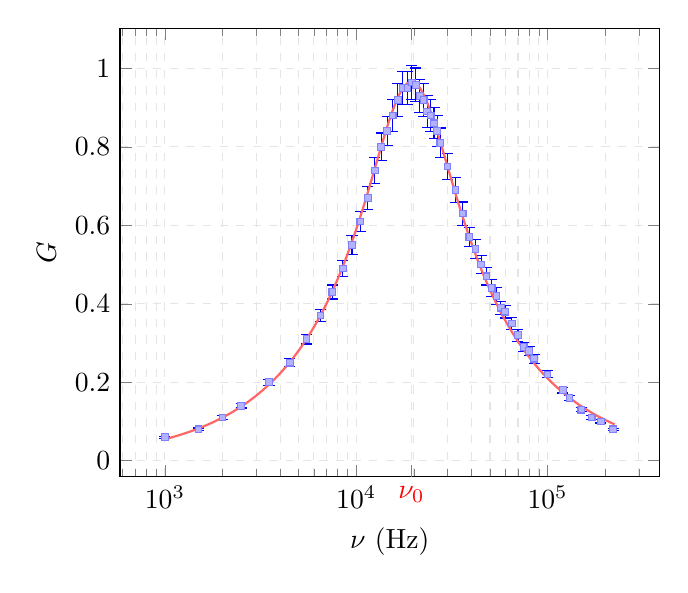
\begin{tikzpicture}
		\begin{axis}[
			%title={Filtro passa-banda RLC},
			xlabel={\(\nu\) (Hz)},
			ylabel={\(G\)},
			grid=both,
			grid style={dashed, gray!20},
			extra x ticks={19429.5},         % Extra tick position (no label yet)
			extra x tick labels={{\color{red}\(\nu_0\)}}, % Label for extra tick
			extra x tick style={         % Style for the extra tick
				grid=major,             % Optional: Add grid line
			},
			xmode=log,
			log basis x=10,
			legend pos=north east
			]
			
			% Dati principali (quadrati blu)
			\addplot+ [
			only marks,
			mark=square*,
			mark options={solid, fill=blue!30, draw=blue!50, scale=0.6},
			error bars/.cd,
			y dir=both,
			y explicit
			] table [y error=error] {
				x       y       error
				1000     0.06     0.00225
				1500     0.08     0.00337
				2000     0.11     0.00453
				2500     0.14     0.00552
				3500     0.20     0.00807
				4500     0.25     0.01001
				5500     0.31     0.01244
				6500     0.37     0.01536
				7500     0.43     0.01791
				8500     0.49     0.02051
				9500     0.55     0.02348
				10500    0.61     0.02620
				11500    0.67     0.02953
				12500    0.74     0.03250
				13500    0.80     0.03526
				14500    0.84     0.03678
				15500    0.88     0.04017
				16500    0.92     0.04155
				17500    0.95     0.04241
				18500    0.95     0.04255
				19500    0.964    0.04313
				20500    0.958    0.04299
				21500    0.93     0.04214
				22500    0.92     0.04173
				23500    0.89     0.04061
				24500    0.88     0.04025
				25500    0.86     0.03954
				26500    0.84     0.03885
				27500    0.81     0.03806
				30000    0.75     0.03284
				33000    0.69     0.03103
				36000    0.63     0.02940
				39000    0.57     0.02472
				42000    0.54     0.02369
				45000    0.50     0.02282
				48000    0.47     0.02212
				51000    0.44     0.02144
				54000    0.42     0.02093
				57000    0.39     0.01657
				60000    0.38     0.01612
				65000    0.35     0.01552
				70000    0.32     0.01511
				75000    0.29     0.01229
				80000    0.28     0.01191
				85000    0.26     0.01164
				100000   0.22     0.00893
				120000   0.18     0.00733
				130000   0.16     0.00702
				150000   0.13     0.00541
				170000   0.11     0.00464
				190000   0.10     0.00396
				220000   0.08     0.00313
			};
			

			\addplot[
			red!60, 
			thick, 
			domain=1000:225000, 
			samples=200
			] {
				285.3/sqrt((285.3 + 10)^2 + (2*pi*x*2.19432e-03 - 1/(2*pi*x*3.05785e-08))^2)
			};
			
		\end{axis}
\end{tikzpicture}
\caption{Set principale con R1}
\end{figure}

Il grafico in figura 2 rappresenta l'andamento del set principale dei nostri dati raccolti in laboratorio. Tale serie risulta essere la più completa a livello di numero di dati.\\
%Questa serie è la più completa che abbiamo raccolto per permetterci di studiare a pieno il comportamento del filtro che abbiamo osservato rispetto alle nostre previsioni teoriche.\\
In aggiunta abbiamo due set con un minor numero di dati ciascuno, che verranno utilizzati per valutare l'influenza della resistenza sulla larghezza di banda:
\begin{figure}[H]
\centering
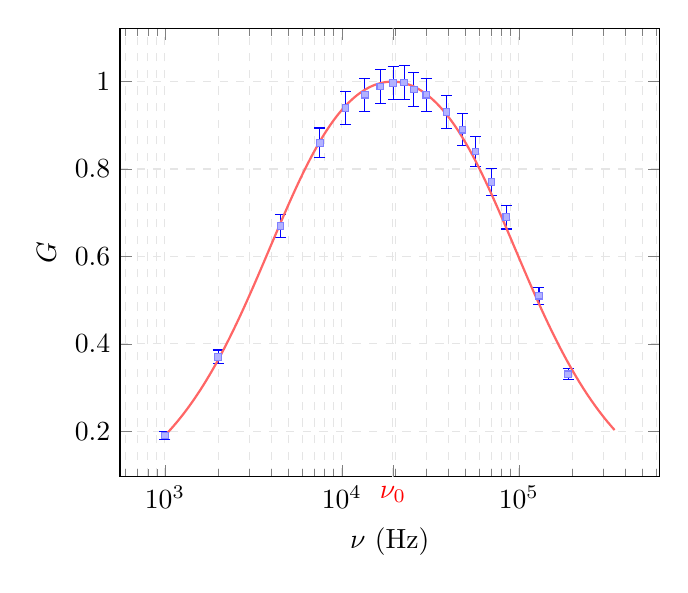
\begin{tikzpicture}
		\begin{axis}[
			xlabel={\(\nu\) (Hz)},
			ylabel={\(G\)},
			grid=both,
			grid style={dashed, gray!20},
			extra x ticks={19429.5},         % Extra tick position (no label yet)
			extra x tick labels={{\color{red}\(\nu_0\)}}, % Label for extra tick
			extra x tick style={         % Style for the extra tick
				grid=major,             % Optional: Add grid line
			},
			xmode=log,
			log basis x=10,
			legend pos=north east
			]
			
			% Dati principali (quadrati blu)
			\addplot+ [
			only marks,
			mark=square*,
			mark options={solid, fill=blue!30, draw=blue!50, scale=0.6},
			error bars/.cd,
			y dir=both,
			y explicit
			] table [y error=error] {
				x       y       error
				1000	0.19	0.00836
				2000	0.37	0.01577
				4500	0.67	0.02583
				7500	0.86	0.03389
				10500	0.94	0.03720
				13500	0.97	0.03804
				16500	0.989	0.03835
				19500	0.997	0.03851
				22500	0.998	0.03865
				25500	0.982	0.03832
				30000	0.97	0.03811
				39000	0.93	0.03723
				48000	0.89	0.03611
				57000	0.84	0.03514
				70000	0.77	0.03063
				85000	0.69	0.02733
				130000	0.51	0.01965
				190000	0.33	0.01270
			};
			

			\addplot[
			red!60, 
			thick, 
			domain=1000:350000, 
			samples=200
			] {
				1020.4/sqrt((1020.4 + 2.33147e-13)^2 + (2*pi*x*2.26305e-03 - 1/(2*pi*x*3.01107e-08))^2)
			};
		\end{axis}
\end{tikzpicture}
\caption{2° set con R2}
\end{figure}
\vspace{-0.5cm}
\begin{figure}[H]
\centering
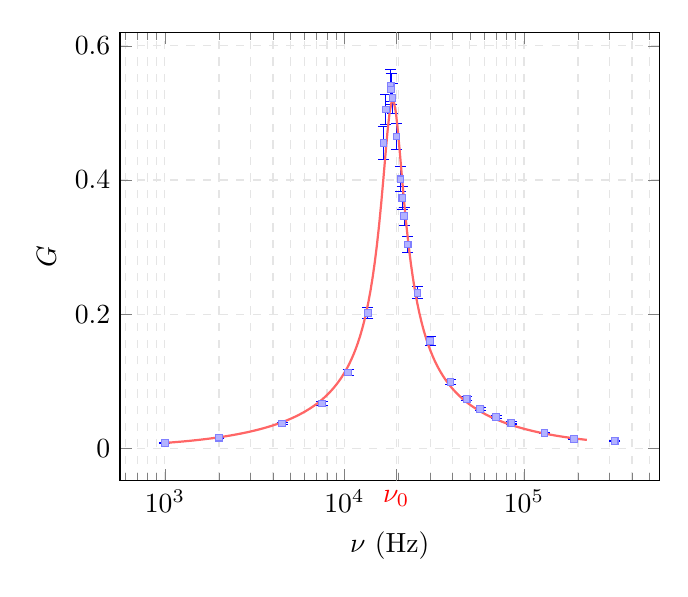
\begin{tikzpicture}
		\begin{axis}[
			xlabel={\(\nu\) (Hz)},
			ylabel={\(G\)},
			grid=both,
			grid style={dashed, gray!20},
			extra x ticks={19429.5},         % Extra tick position (no label yet)
			extra x tick labels={{\color{red}\(\nu_0\)}}, % Label for extra tick
			extra x tick style={         % Style for the extra tick
				grid=major,             % Optional: Add grid line
			},
			xmode=log,
			log basis x=10,
			legend pos=north east
			]
			
			% Dati principali (quadrati blu)
			\addplot+ [
			only marks,
			mark=square*,
			mark options={solid, fill=blue!30, draw=blue!50, scale=0.6},
			error bars/.cd,
			y dir=both,
			y explicit
			] table [y error=error] {
				x       y       error
				1000	0.008	0.00032
				2000	0.016	0.00062
				4500	0.037	0.00143
				7500	0.067	0.00256
				10500	0.113	0.00437
				13500	0.202	0.00835
				16500	0.455	0.02466
				17000	0.505	0.02244
				18100	0.541	0.02344
				18200	0.535	0.02310
				18500	0.522	0.02247
				19500	0.465	0.01904
				20500	0.401	0.01860
				21000	0.373	0.01679
				21500	0.346	0.01324
				22500	0.304	0.01166
				25500	0.232	0.00866
				30000	0.160	0.00620
				39000	0.099	0.00374
				48000	0.074	0.00273
				57000	0.059	0.00219
				70000	0.047	0.00173
				85000	0.038	0.00155
				130000	0.023	0.00088
				190000	0.014	0.00054
				320000	0.011	0.00040
			};
			
			
			\addplot[
			red!60, 
			thick, 
			domain=1000:225000, 
			samples=200
			] {
				40.69/sqrt((40.69 + 3.76712e+01)^2 + (2*pi*x*2.28532e-03 - 1/(2*pi*x*3.21116e-08))^2)
			};
			
		\end{axis}
\end{tikzpicture}
\caption{3° set con R3}
\end{figure}
Per ogni set di dati è stato svolto un fit con il metodo dei minimi quadrati e sono stati ricavati i valori di capacità, induttanza e resistenza parassita; in particolare per il primo set di dati abbiamo ottenuto:
\begin{table}[H]
    \centering
    \begin{tabular}{c c c}
    \hline
    $C_{F1}$ & $30.6 \pm 0.9$ & nF \\
    $L_{F1}$ & $2.20 \pm 0.06$ & mH \\
    $R_{parF1}$& $11 \pm 3$ & $\Omega$ \\
    $\nu_{0F1}$& $19408 \pm 389$ & Hz \\
    \hline
\end{tabular}
\caption{Dati del fit di Fig. 1}
\end{table}
Confrontando\footnote{Per i confronti sono stati usati opportuni test di gauss, svolti confrontando la differenza dei rispettivi parametri con il valore atteso, ovvero 0} i parametri circuitali ottenuti dai fit con i valori misurati in laboratorio abbiamo ottenuto corrispondenze interessanti: I valori di capacità sono risultati molto concordi fra loro, con un P-value pari a 0.50; invece le induttanze sono confrontabili fra di loro ma con un P-value pari a 0.08.
\`E interessante notare però che i valori di L sono estremamente compatibili fra i tre set di dati, quindi sembra esserci una leggera discordanza fra il valore misurato con il ponte e il valore che risulta dal comportamento del filtro. \`E quindi probabile che ci sia una ragione per cui misuriamo con il ponte un valore di L inferiore a quello vero.\\ 

Questa differenza fra i valori di L si riflette anche sulla frequenza di risonanza, che continua ad essere compatibile con quella ottenuta direttamente dalle grandezze misurate, ma diminuisce di 0.6 KHz. Questa non è una differenza trascurabile: constatiamo che un valore più veritiero della $\nu_0$ del nostro circuito è quello che otteniamo dal primo fit; infatti il valore di frequenza a cui abbiamo misurato il guadagno massimo in laboratorio è stato 19500 Hz. \\
In aggiunta si può vedere come per il primo set di dati la resistenza parassita sia piccola ma non nulla, ed il suo effetto non è trascurabile nell'andamento del filtro. Questo valore di $R_{parF1}$ è il motivo per cui il guadagno massimo della fig. 2 si discosta dall'1. Mentre per il secondo fit, la cui resistenza è molto maggiore, l'effetto della resistenza parassita è trascurabile ed il guadagno massimo è molto vicino ad 1.\\

Si evidenzia inoltre che a partire da circa 350 KHz i dati di tutti e tre i set presentano deviazioni anomale rispetto all'andamento previsto. Questo comportamento può essere attribuito alla forte attenuazione del segnale al di fuori della banda passante del filtro, che rende la misura più sensibile a rumori di fondo. L'effetto non è attribuibile all'impedenza d'ingresso dell'oscilloscopio poichè la frequenza di taglio del circuito RC interno si trova a frequenze molto più alte, circa 8 MHz.\\

Le figure 3 e 4 mettono in risalto l'effetto della resistenza sulla larghezza di banda passante. Come previsto dalla formula teorica la proporzionalità è diretta; infatti per una resistenza maggiore la banda si allarga, mentre per una resistenza più piccola si stringe. \'E opportuno far notare che per la Fig. 4 la larghezza di banda è talmente piccola che in laboratorio non siamo riusciti a trovare i valori di frequenza per cui il guadagno fosse maggiore di 0.53, si può calcolare infatti che la larghezza di banda in questo caso risulta all'incirca di 300 Hz, mentre per la Fig. 3 è all'incirca 7.7 KHz. Inoltre, come già discusso in precedenza, la resistenza parassita del circuito è piccola; ma per il terzo set anche la resistenza che abbiamo scelto è molto piccola, di conseguenza anche questa scelta contribuisce ad abbassare il picco del guadagno.\\
    
\section{Conclusioni}
Giunti a questo punto possiamo asserire che l'obbiettivo dell'analisi dati è stato raggiunto: abbiamo caratterizzato la risposta in frequenza di un circuito RLC.\\
Tramite i confronti con i valori dei fit abbiamo riscontrato un possibile errore sistematico sulla misura dell'induttanza, della quale consideriamo come valore più accurato quello ottenuto dai fit, ovvero $2.20 \pm 0.06$ mH. Questo offset sul valore di L si ripercuote sulla $\nu_0$, che consideriamo essere $19.4 \pm 0.4$ kHz, ovvero il valore ottenuto dal fit di Fig. 2. Infine abbiamo valutato come il valore della resistenza del circuito influenzasse la larghezza di banda, confermando la formula teorica.

\end{document}